\documentclass[12pt,twoside]{article}
%%%%%%%%%%%%%%%%%%%%%%%%%%%%%%%%%%%%%%%%%%%%%%%%%%%%%%%%%%%%%
% Meta informations:
\newcommand{\trauthor}{Jan Fabian Schmid}
\newcommand{\trtype}{Seminar Paper} %{Seminararbeit} %{Proseminararbeit}
\newcommand{\trcourse}{Bio-inspired Artificial Intelligence}
\newcommand{\trtitle}{Effects of encoding on the general learning ability of artificial neural networks}
\newcommand{\trmatrikelnummer}{6440383}
\newcommand{\tremail}{2schmid@informatik.uni-hamburg.de}
\newcommand{\trarbeitsbereich}{Knowledge Technology, WTM}
\newcommand{\trdate}{16.12.2015}

%%%%%%%%%%%%%%%%%%%%%%%%%%%%%%%%%%%%%%%%%%%%%%%%%%%%%%%%%%%%%
% Languages:

% Falls die Ausarbeitung in Deutsch erfolgt:
% \usepackage[german]{babel}
% \usepackage[T1]{fontenc}
% \usepackage[latin1]{inputenc}
% \usepackage[latin9]{inputenc}	 				
% \selectlanguage{german}

% If the thesis is written in English:
\usepackage[english]{babel} 						
\selectlanguage{english}

%%%%%%%%%%%%%%%%%%%%%%%%%%%%%%%%%%%%%%%%%%%%%%%%%%%%%%%%%%%%%
% Bind packages:
\usepackage{acronym}                    % Acronyms
\usepackage{algorithmic}								% Algorithms and Pseudocode
\usepackage{algorithm}									% Algorithms and Pseudocode
\usepackage{amsfonts}                   % AMS Math Packet (Fonts)
\usepackage{amsmath}                    % AMS Math Packet
\usepackage{amssymb}                    % Additional mathematical symbols
\usepackage{amsthm}
\usepackage{booktabs}                   % Nicer tables
%\usepackage[font=small,labelfont=bf]{caption} % Numbered captions for figures
\usepackage{color}                      % Enables defining of colors via \definecolor
\definecolor{uhhRed}{RGB}{254,0,0}		  % Official Uni Hamburg Red
\definecolor{uhhGrey}{RGB}{122,122,120} % Official Uni Hamburg Grey
\usepackage{fancybox}                   % Gleichungen einrahmen
\usepackage{fancyhdr}										% Packet for nicer headers
%\usepackage{fancyheadings}             % Nicer numbering of headlines

%\usepackage[outer=3.35cm]{geometry} 	  % Type area (size, margins...) !!!Release version
%\usepackage[outer=2.5cm]{geometry} 		% Type area (size, margins...) !!!Print version
%\usepackage{geometry} 									% Type area (size, margins...) !!!Proofread version
\usepackage[outer=3.15cm]{geometry} 	  % Type area (size, margins...) !!!Draft version
\geometry{a4paper,body={5.8in,9in}}

\usepackage{graphicx}                   % Inclusion of graphics
%\usepackage{latexsym}                  % Special symbols
\usepackage{longtable}									% Allow tables over several parges
\usepackage{listings}                   % Nicer source code listings
\usepackage{multicol}										% Content of a table over several columns
\usepackage{multirow}										% Content of a table over several rows
\usepackage{rotating}										% Alows to rotate text and objects
\usepackage[hang]{subfigure}            % Allows to use multiple (partial) figures in a fig
%\usepackage[font=footnotesize,labelfont=rm]{subfig}	% Pictures in a floating environment
\usepackage{tabularx}										% Tables with fixed width but variable rows
\usepackage{url,xspace,boxedminipage}   % Accurate display of URLs

%%%%%%%%%%%%%%%%%%%%%%%%%%%%%%%%%%%%%%%%%%%%%%%%%%%%%%%%%%%%%
% Configurationen:

\hyphenation{whe-ther} 									% Manually use: "\-" in a word: Staats\-ver\-trag

%\lstloadlanguages{C}                   % Set the default language for listings
\DeclareGraphicsExtensions{.pdf,.svg,.jpg,.png,.eps} % first try pdf, then eps, png and jpg
\graphicspath{{./src/}} 								% Path to a folder where all pictures are located
\pagestyle{fancy} 											% Use nicer header and footer

% Redefine the environments for floating objects:
\setcounter{topnumber}{3}
\setcounter{bottomnumber}{2}
\setcounter{totalnumber}{4}
\renewcommand{\topfraction}{0.9} 			  %Standard: 0.7
\renewcommand{\bottomfraction}{0.5}		  %Standard: 0.3
\renewcommand{\textfraction}{0.1}		  	%Standard: 0.2
\renewcommand{\floatpagefraction}{0.8} 	%Standard: 0.5

% Tables with a nicer padding:
\renewcommand{\arraystretch}{1.2}

%%%%%%%%%%%%%%%%%%%%%%%%%%%%
% Additional 'theorem' and 'definition' blocks:
\theoremstyle{plain}
\newtheorem{theorem}{Theorem}[section]
%\newtheorem{theorem}{Satz}[section]		% Wenn in Deutsch geschrieben wird.
\newtheorem{axiom}{Axiom}[section] 	
%\newtheorem{axiom}{Fakt}[chapter]			% Wenn in Deutsch geschrieben wird.
%Usage:%\begin{axiom}[optional description]%Main part%\end{fakt}

\theoremstyle{definition}
\newtheorem{definition}{Definition}[section]

%Additional types of axioms:
\newtheorem{lemma}[axiom]{Lemma}
\newtheorem{observation}[axiom]{Observation}

%Additional types of definitions:
\theoremstyle{remark}
%\newtheorem{remark}[definition]{Bemerkung} % Wenn in Deutsch geschrieben wird.
\newtheorem{remark}[definition]{Remark} 

%%%%%%%%%%%%%%%%%%%%%%%%%%%%
% Provides TODOs within the margin:
\newcommand{\TODO}[1]{\marginpar{\emph{\small{{\bf TODO: } #1}}}}

%%%%%%%%%%%%%%%%%%%%%%%%%%%%
% Abbreviations and mathematical symbols
\newcommand{\modd}{\text{ mod }}
\newcommand{\RS}{\mathbb{R}}
\newcommand{\NS}{\mathbb{N}}
\newcommand{\ZS}{\mathbb{Z}}
\newcommand{\dnormal}{\mathit{N}}
\newcommand{\duniform}{\mathit{U}}

\newcommand{\erdos}{Erd\H{o}s}
\newcommand{\renyi}{-R\'{e}nyi}
%%%%%%%%%%%%%%%%%%%%%%%%%%%%%%%%%%%%%%%%%%%%%%%%%%%%%%%%%%%%%
% Document:
\begin{document}
\renewcommand{\headheight}{14.5pt}

\fancyhead{}
\fancyhead[LE]{ \slshape \trauthor}
\fancyhead[LO]{}
\fancyhead[RE]{}
\fancyhead[RO]{ \slshape \trtitle}

%%%%%%%%%%%%%%%%%%%%%%%%%%%%
% Cover Header:
\begin{titlepage}
	\begin{flushleft}
		Universit\"at Hamburg\\
		Department Informatik\\
		\trarbeitsbereich\\
	\end{flushleft}
	\vspace{3.5cm}
	\begin{center}
		\huge \trtitle\\
	\end{center}
	\vspace{3.5cm}
	\begin{center}
		\normalsize\trtype\\
		[0.2cm]
		\Large\trcourse\\
		[1.5cm]
		\Large \trauthor\\
		[0.2cm]
		\normalsize Matr.Nr. \trmatrikelnummer\\
		[0.2cm]
		\normalsize\tremail\\
		[1.5cm]
		\Large \trdate
	\end{center}
	\vfill
\end{titlepage}

	%backsite of cover sheet is empty!
\thispagestyle{empty}
\hspace{1cm}
\newpage

%%%%%%%%%%%%%%%%%%%%%%%%%%%%
% Abstract:

% Abstract gives a brief summary of the main points of a paper:
\section*{Abstract}
 TODO

% Lists:
\setcounter{tocdepth}{2} 					% depth of the table of contents (for Seminars 2 is recommented)
\tableofcontents
\pagenumbering{arabic}
\clearpage

%%%%%%%%%%%%%%%%%%%%%%%%%%%%
% Content:

% the actual content, usually separated over a number of sections
% each section is assigned a label, in order to be able to put a
% crossreference to it

\section{Introduction}
\label{sec:introduction}
This seminar paper is supposed to give an in-depth analysis of the presented paper \cite{citeulike:12788284} with focus on the effects of encoding on the general learning ability of artificial neural networks.\medskip
One of the more prominent topics in bio-inspired artificial intelligence is the modelling of animal nervous systems using artificial neural networks (ANNs) (cf. \cite{citeulike:12788284} p.1).\\
ANNs are used for function approximation in a variety of application fields.
In contrast to them nature-like neural networks should be larger, more organized and more plastic (cf. \cite{citeulike:12788284} p.1). 
The common approach to develope such networks, are evolutionary algorithms, since the evolution was responsible for developing the prototype.\\
Two aspects of creating nature-like ANNs, that research mainly focuses on, are:
\begin{itemize}
	\item \textbf{Genetic encoding:} To use evolutionary algorithms for the developement of neural networks with specific behaviours, it is necessary to present the structure in some kind of encoding that can be handled by them.
	As in the genotype of animals, it is not desired to encode each neuron specifically, but rather to define rules for the network structure, that then lead to regular patterns (cf. \cite{citeulike:12788284} p.1).\\
	Algorithms that use a mapping of genotype to phenotype are called \textit{artificial developmental systems}.
	\item \textbf{Synaptic plasticity:} The ability of an artificial neural network to change repeatedly during lifetime is called synaptic plasticity.
	A neural network with good plasticity is supposed to be able to adapt to different problems through a learning process, ideally even to situations that were not considered during the developement of the network.
\end{itemize}
Alongside a proper genetic encoding the fitness function has to be defined for evolutionary algorithms. Individuals that are newly developed during the application of the algorithm are adapted to the fitness function. \\
To obtain plastic ANNs the fitness function could check for fitness on many different test cases to ensure the general learning ability.
It turns out however that this approach can hardly be feasible for more complex environments as the number of required test cases grows exponentially (cf. \cite{citeulike:12788284} p.2).\medskip
In the studied paper \cite{citeulike:12788284} it is therefore suggested that genetic encoding and synaptic plasticity should be examined simultaneously (cf. \cite{citeulike:12788284} p. 1).\\

\subsection{Hypothesis}
Tonelli and Mouret say that the use of artificial developmental systems leads to more regular network structures since it is easier to describe a more regular structure with repetitions and symmetries than to describe an irregular structure with seemingly no relations between the induvidual network parts using a general rule set like genetic encoding does.(cf. \cite{citeulike:12788284} p.2)
Therefore their main hypothesis is:
\glqq We here propose that this bias towards regularity is critical to evolve plastic neural networks that can learn in a large variety of situations\grqq{}(\cite{citeulike:12788284} p.2).\\
To visualize this idea they present the illustration in figure (\textbf{???}).

\begin{figure}
	\begin{center}
		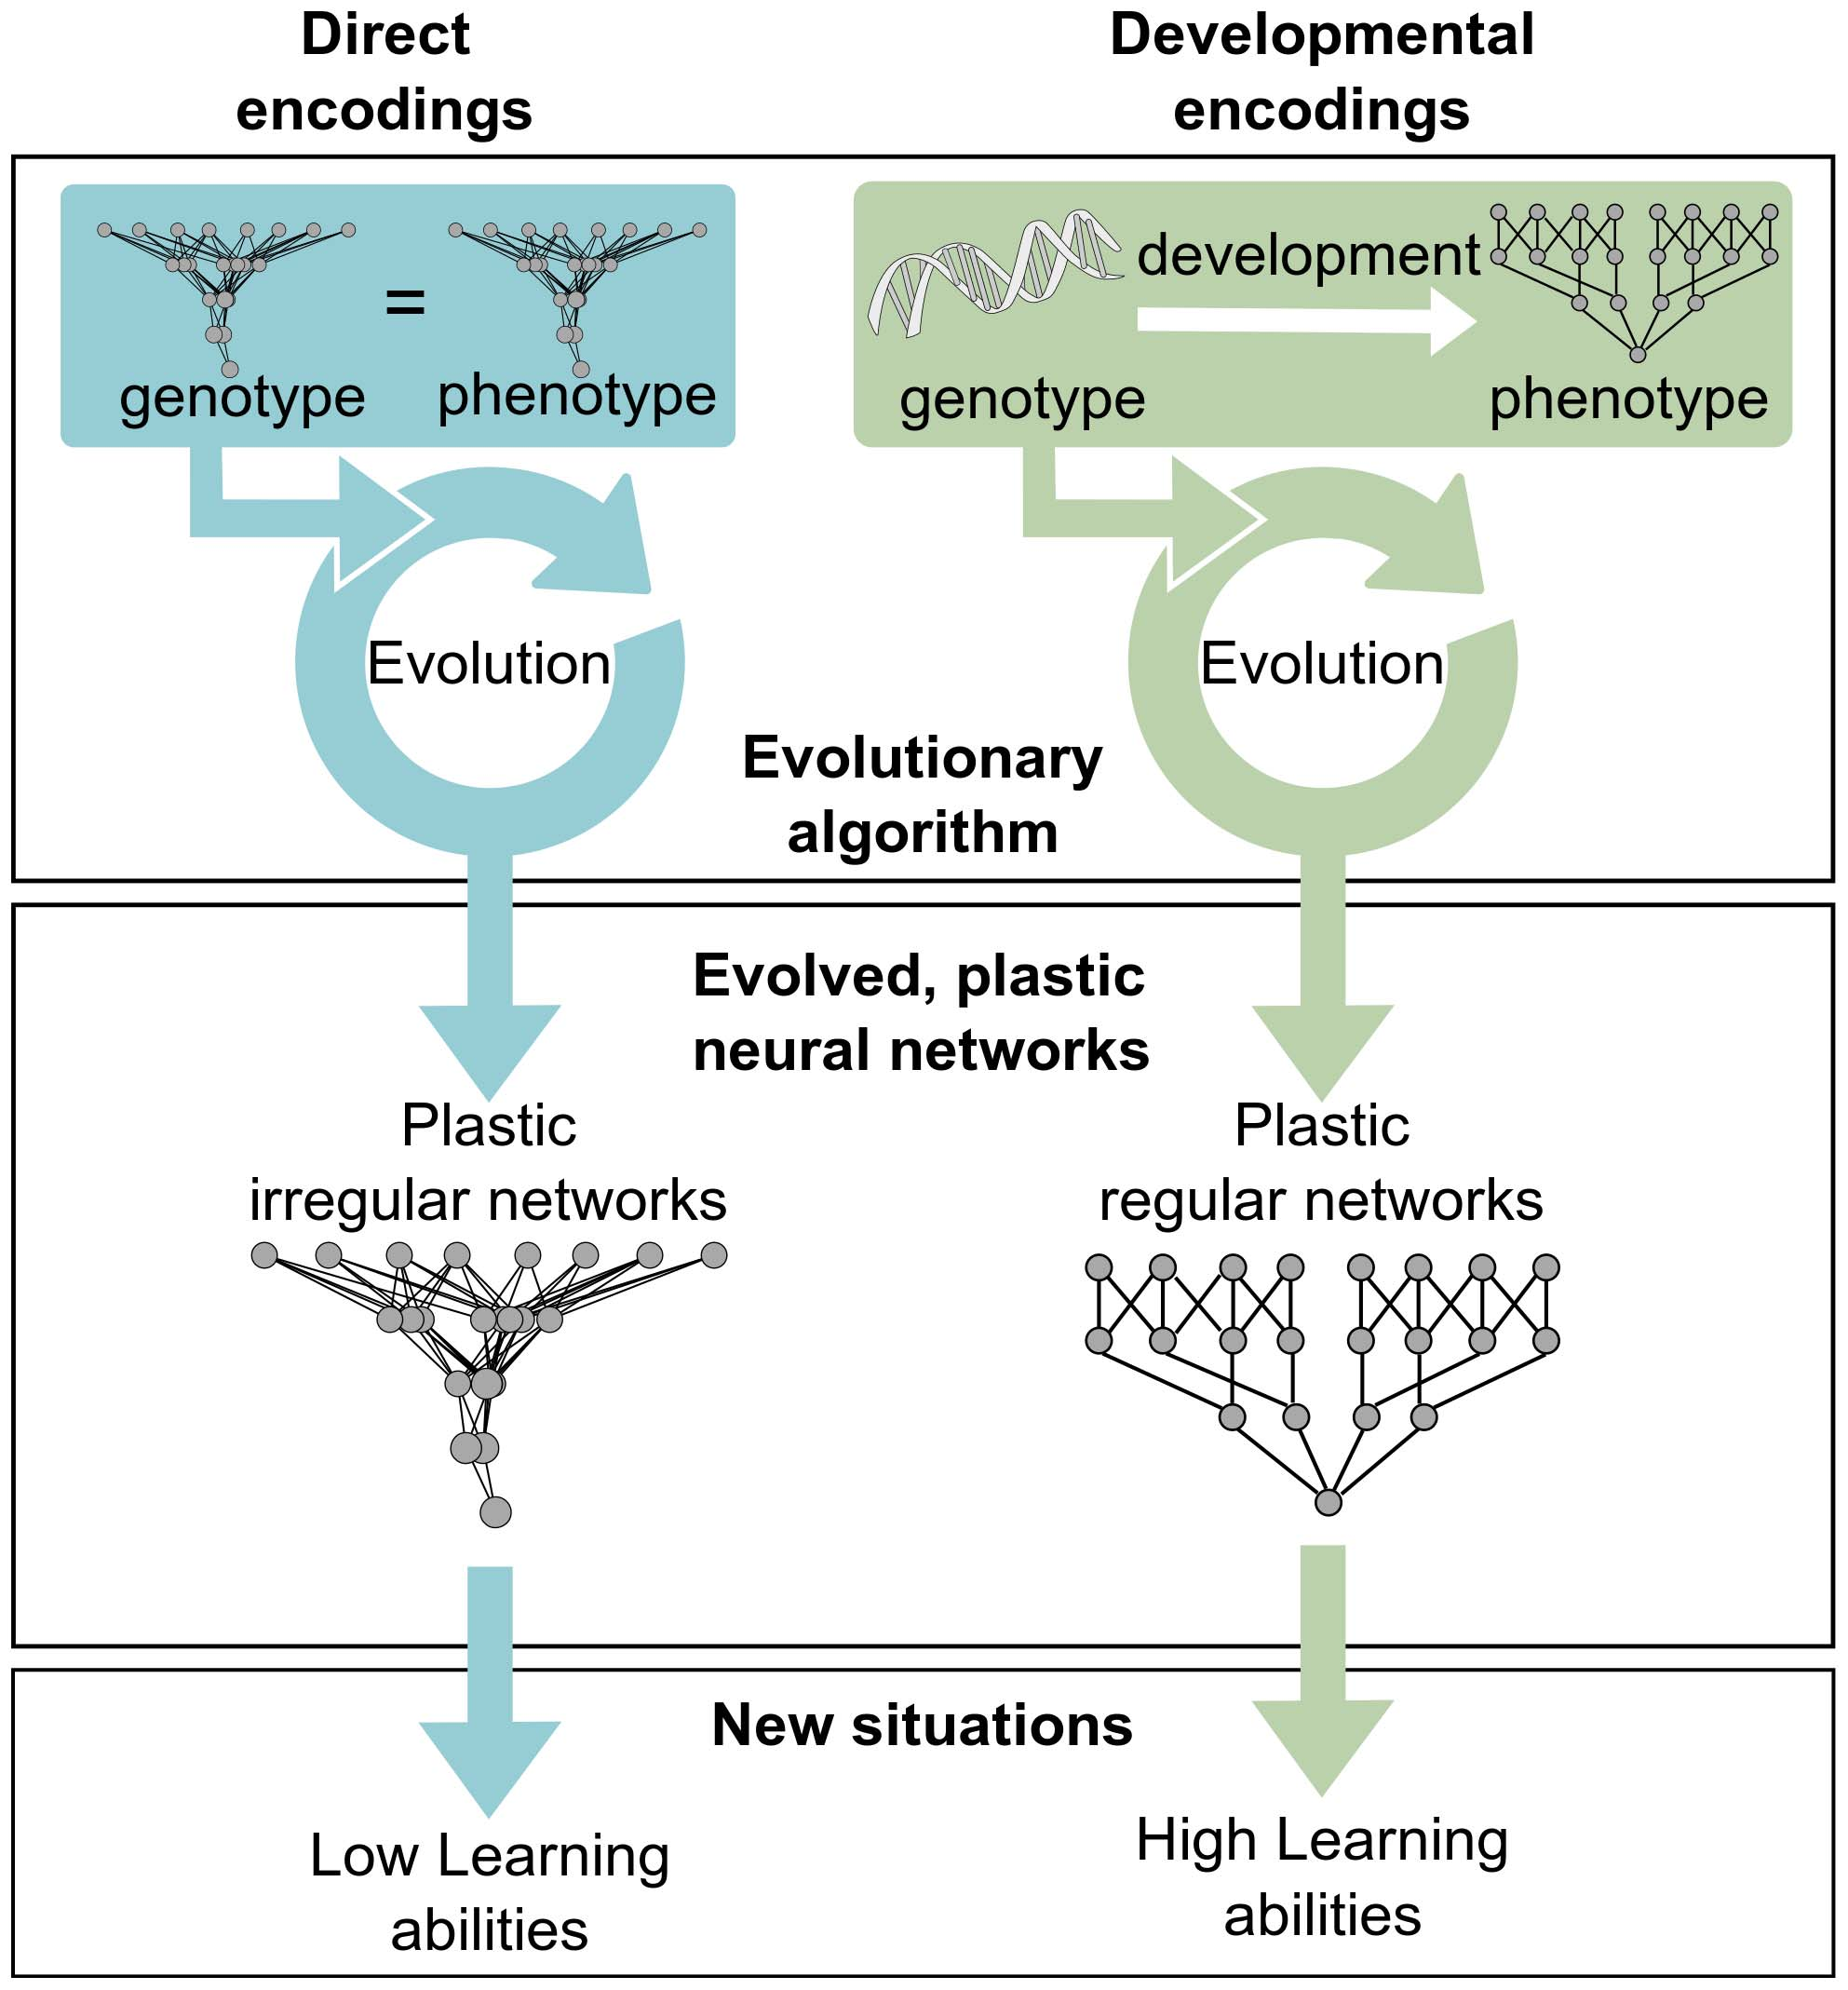
\includegraphics[totalheight=0.4\textheight]{direct_vs_developemental.png}
		\caption[\textbf{Main hypothesis.} Using developmental encodings should facilitate the evolution of plastic ANNs with high learning abilities.
		\text{doi:10.1371/journal.pone.0079138.g001}]{\textbf{Main hypothesis.} Using developmental encodings should facilitate the evolution of plastic ANNs with high learning abilities.
			\text{doi:10.1371/journal.pone.0079138.g001} \footnotemark} %
	\end{center}
\end{figure}
\footnotetext{Source: Tonelli, Paul and Mouret, Jean-Baptiste (2013), \cite{citeulike:12788284} p.3}

The better general learning ability of more regular ANNs is supposed to stem from higher redundancies of network parts as the ANN can't be as specialized to the specific test cases used by the fitness function as a direct encoded network would be.

%\subsection{Goals and structure of this paper}
%In chapter \ref{sec:background} some background information necessary to understand the concepts and the experimental setup used in the discussed paper will be given.
%Then in chapter \ref{sec:related_work} related publications that use artificial developmental systems for the developement of nature-like ANNs are presented.
%A description of how the proposed hypothesis was tested will be covered by chapter \ref{sec:model}.
%Following, the results and conclusions are discussed in chapter \ref{sec:analysis}.
%Then chapter \ref{sec:concl} will conclude the paper by summarizing the main findings.

\section{Background Information}
\label{sec:background}

\subsection{subject index (Stichwortverzeichnis)}
Phenotype, Genotype, 

%Evolutionary algorithms
\subsection{Regularity}
\label{regularity}
Regularity measures the compressibility of a network. It is a characterization of the phenotype, not the genotype, of the ANN.
Tonelli and Mouret compute the regularity by calculating the number of symmetry axes (cf. \cite{citeulike:12788284} p. 4).
If two parts of the network can be interchanged without altering the graph they are called symmetric.
It is only necessary to describe one of these parts and reference it for each additional occurance, therefore the description of a network with more symmetries is more compressable.\\
These symmetries are graph automorphisms and can be easily calculated for most graphs (actually it is an NP-complete problem).\\
A graph automorphism is a permutation $\sigma$ of the vertex set V of the graph $G = (V,E)$, that maps an edge $(\sigma(u),\sigma(v))$ to the vertices u and v iff they formed an edge (u,v) already in G.\\
Since an automorphism of the graph to itself always exists, the number of symmetries is the number of automorphisms less one.

\subsection{From genes to nervous systems}
\label{genes_nervous}
It is necessary to encode the structure of an ANN to a representation that can be modified easily if an evolutionary algorithm is to be used for its developement.
Encodings can be divided into two groups:
\begin{itemize}
	\item \textbf{Developemental encodings} use a genotype to phenotype mapping like DNA does. The code defines construction rules which if followed lead to a certain network structure. Small changes in the code can, if followed, have huge impacts on the resulting phenotype allowing a fast exploration of parameter space, but the fine tuning becomes difficult.
	Often similar and symmetric network structure parts arise in the phenotype since all neurons, and all connections, follow the same rules.
	\item For \textbf{direct encodings} the mapping from genotype to phenotype is immediate as the parameters to each neuron and each connection can be directly derived from the code. In the developemental encoding this is not possible since they depend on their relation to different network parts by the defined rules.
\end{itemize}
In the studied paper three different encodings are compared with each other, two of them are developemental encodings (HNN and map-based) and one direct encoding.

\subsubsection{Direct encoding}
The ANN is decribed by a directed graph. The networks of the first generation of the evolutionary algorithm are initiated as a simple feed-forward network without hidden layers and randomly initialized weights.\\
Seven different mutation operators are modifying the network during evolution while no cross over is implemented in the version used by Tonelli and Mouret (cf. \cite{citeulike:12788284} p. 9-10).
Each mutation happens with a specific probability to the operation:
\begin{itemize}
	\item A connection is randomly added
	\item A random connection is removed
	\item Randomly choose a connection and change its target or source
	\item Create a new neuron by randomly choosing a connection and creating a new target neuron with the same connection weight
	\item Delete a random neuron and its connections
	\item Randomly choose a connection and modify its weight
	\item Activation function of a random neuron is changed
\end{itemize}

\subsubsection{map-based encoding}
The map-based encoding develops a network structure in a similar way as the direct encoding does, but instead of directly setting neurons and their connections, nodes and edges are used.
Nodes and Edges of the developed neural net are however encoded in a specific, more complex way. Because of this part of the encoding it doesn't behave as a direct encoding, but as a developmental encoding.\\
Each node of the network represents a whole map of neurons. A map of neurons is an array of $N \times M$ identical neurons and is defined by a set of parameters (??? \cite{tonelli2011using} p. 3). 
In the map-based encoding in the studied paper each parameter value is a real number between 0 and 1 and is mutated during the evolutionary process.
The meaning of an parameter 'flips' by exceeding a certain value (for example: a parameter value between 0 and 0.4 means 'a' and 'b' for a value between 0.4 and 1).
One parameter of the neuron map for example decides if it represents only a single neuron or a set array size of neurons.\\
The edges between maps are described as well with a number of parameters.
In this case the type of connection and the synaptic weight are set by parameters.
One parameter decides if each neuron of a map is only connected to one neuron of the map on the other side of the edge or if each neuron is connected to each other neuron.
Another parameter implies if the connection weights have positive or negative sign (excitatory or inhibitory). And the last parameter sets the weight value.

\subsubsection{HNN encoding}
The Hyper Neural Network (HNN) encoding used by Tonelli and Mouret is a modification of the complex HyperNEAT encoding.
When using this encoding the network structure has to be specified beforehand (in this case 9 input neurons, 5 hidden neurons and 4 output neurons).
During the evolutionary development of the network two additional included networks are formed. One of them answers the question to each pair of neurons, if they are connected or not and if so which connection weight the edge has.
The second inherent network defines the parameters of each neuron. These two networks are developed using the direct encoding.
Through the interaction of the two inherent networks with the given main-network structure a the HNN encoding meets the requirements of a developmental encoding.

\subsection{Skinner box}
A Skinner box is a typical experiment to test the learning ability of an animal (usually rats).
The standard configuration of a Skinner box can be seen in figure \ref{fig:skinner}, it can be described with input and output items.
The test animal has to associate the inputs with the	appropriate output.
As stimuli input, lights or sounds from a loudspeaker might be used. The test animal is then supposed to press the associated response lever according to the stimulus.
The association patterns are set arbitrarily by the experimenter. For example the test animal might be supposed to push the lever (as output) if the green light appears, but not if the red light shines.
As additional input the food dispenser and electrified grid can then be used to support the 'right' behaviour and/or punish the 'wrong' behaviour.

\begin{figure}[h]
	\begin{center}
		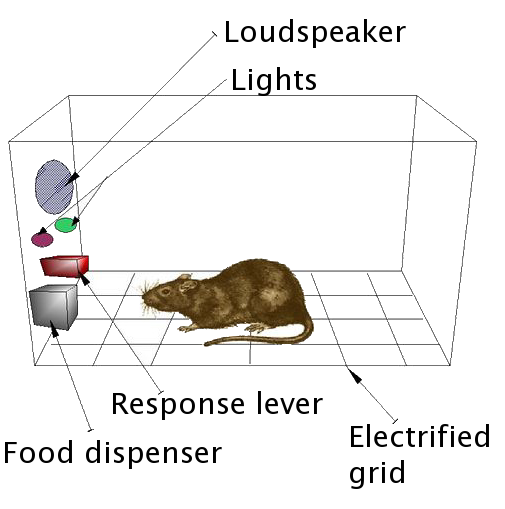
\includegraphics[width=.43\textwidth]{Skinner_box_scheme_01.png}
	\end{center}
	\caption{Skinner box, wiki}
	\label{fig:skinner}
\end{figure}

A test animal (or different test subject) with good general learning ability, should be able to identify the supported input to output associations independent of the specific used pairing and act accordingly.

%\section{TODO: related work}
%\label{sec:related_work}
%Typical approaches from related work\\
%- typically the two problems ( 1. encoding of nervous systems for evolution of %large good neural networks and 2. synaptic plasticity in neural networks) are %studied separately\\
%About generative encodings: \\
%- \cite{hornby2001body} $\rightarrow$ L-Systems\\
%- \cite{mouret2010importing} $\rightarrow$ neuroscience toolbox\\
%About synaptic plasticity:\\
%- \cite{hebb2005organization} $\rightarrow$ importance of synaptic plasticity for %learning\\
%- \cite{abbott2000synaptic} $\rightarrow$ synaptic plasticity in neural networks

\section{Approach description}
\label{sec:model}
%Experiment in the paper to verify the proposal - design of analysis\\
%- What kind of simplifications were made for this approach?\\
To test their hypothesis, that developmental encodings lead to ANNs with better general learning ability, Tonelli and Mouret used the following experimental setup:\medskip

Developed ANNs are trained and tested in a simulated Skinner box with four stimuli inputs (1,2,3,4) and also four possible output actions (A,B,C,D). Only one stimulus is presented at once and is associated with one desired output action.
For further consideration four terms are defined by Tonelli and Mouret:
\begin{itemize}
	\item A \textbf{association} (I,O) is a pair of input stimulus and output action, where the input I should lead to the output O (e.g. (1,A)).
	\item The \textbf{association set} is a set with one association to each input simulus (e.g. $\left\{(1,A),(2,B),(3,C),(4,D)\right\})$
	\item The \textbf{global training set} is the set of all possible association sets (with four different stimuli and four possible actions there are $4^4 = 256$ different possibilities).
	\item The \textbf{evolutionary training set} is a randomly chosen subset of the global training set, that is used during a particular experiment to evaluate the general leraning ability of the evolved ANNs.
	\item With the \textbf{General Learning Ability} (GLA) score the performance of an evolved ANN on all association sets, that were not used during the evolutionary process.
\end{itemize}

The ANNs that are developed have ten input and four output nodes. Four input nodes for the four possible input stimuli, four for a copy of the last output of the ANN and one each for reward and punishment.
The figure \ref{fig:formalization} shows an illustration of the network structure.

\begin{figure}[h]
	\begin{center}
		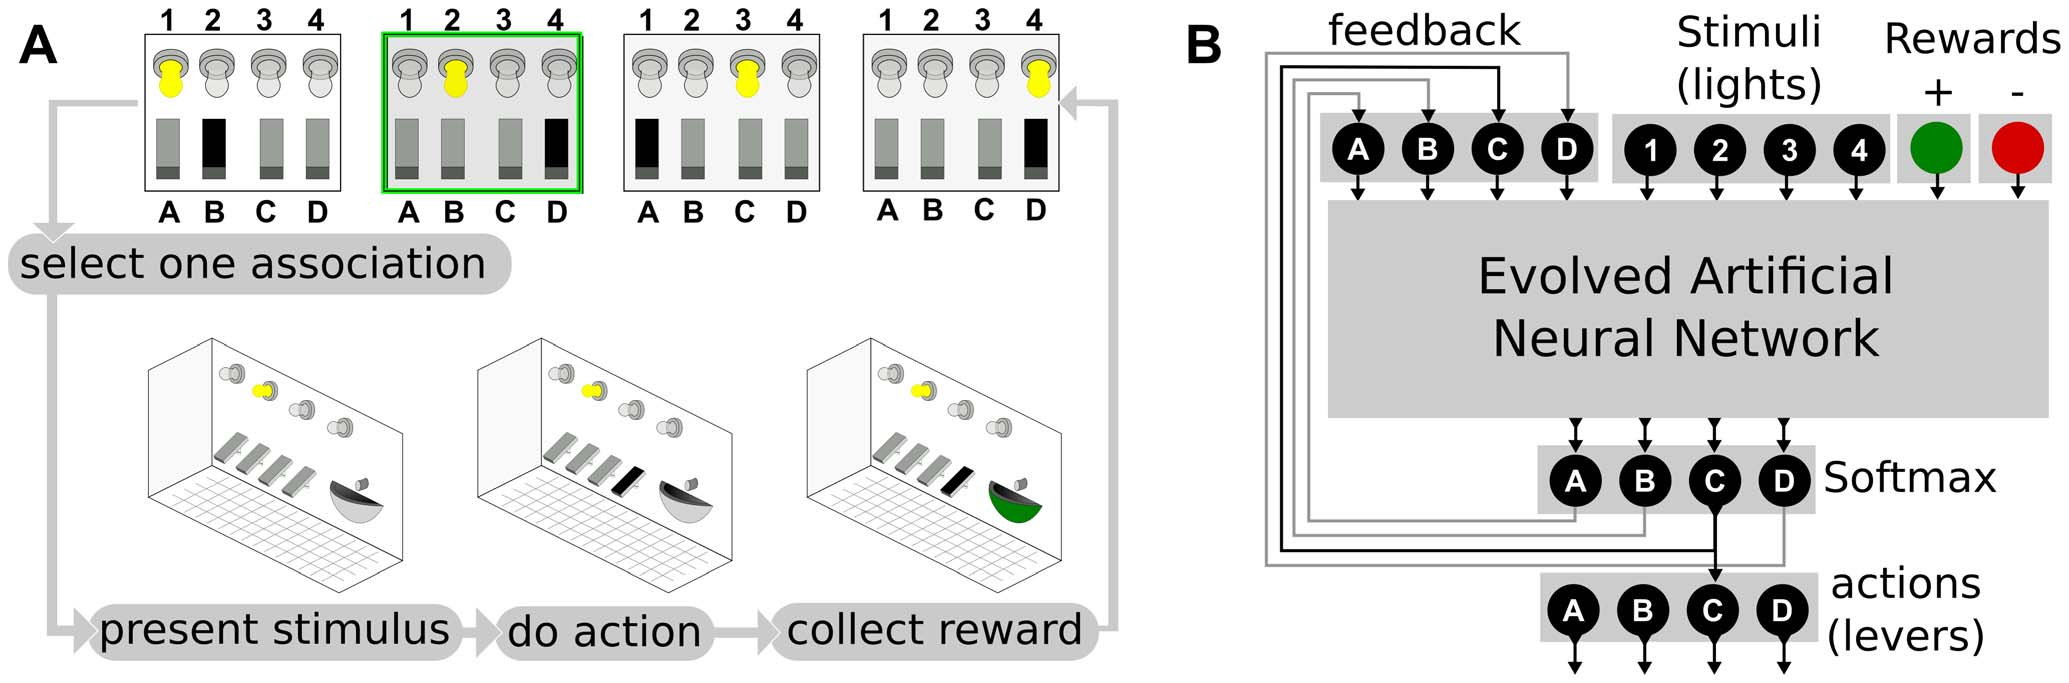
\includegraphics[width=.9\textwidth]{network_structure.png}
	\end{center}
	\caption{Formalizastion of the Skinner box as a task for an artificial neural network. Abschneiden!}
	\label{fig:formalization}
\end{figure}

To calculate the answer of the ANN to an input the softmax of the output values is taken. The softmax in contrast to the simple max function does not just take the output node with the highest value as answer of the ANN, but assigns a probability to be taken proportional to the quantity of a value (higher value leads to higher likelyhood to be choosen as final answer).\medskip

Example of input/outoput values to the network (abbildung maipulieren)\medskip

The learning process of an ANN to a association set is not done with classical backpropagation and corresponding weight changes, but by using modulatory neurons.
Each neuron in the ANN can be a standard or a modulatory one.
Modulatory neurons change the connection weights of standard neurons using Hebb's rule ("Cells that fire together, wire together") and induce thereby plasticity to the ANN (cf. \cite{citeulike:12788284} p.2).\\
Beispiel wie das funktionieren kann, zeigen. Mehrere Iterationen führen zu jeweils utnerschiedlicher modulation der gewichte bis irgendwann das korrekte ergebnis erscheint. \medskip

To start a new experiment a subset of the global training set is randomly chosen as evolutionary training set.
An evolutionary algorithm is then used to create ANNs with good performance on the training set for each of the three different genetic encodings studied by Tonelli and Mouret : direct, map-based and HNN encoding. As the name suggests direct encoding is a representative of the direct encodings introduced in chapter \ref{genes_nervous}, whereas map-based and HNN encoding are among the developemental encodings.
The 'Non-dominated Sorting Genetic Algorithm-II' (NSGA-II) a multi-objective optimization algorithm, that utilizes evolutionary methods, is the selected evolutionary algorithm by Tonelli and Mouret for their experiments.\\
It is necessary to define a fitness function, to evaluate the performance of individuals during the evolutionary process. The fitness function used by Tonelly and Mouret does the following:\\
First an association set of the evolutionary training set is chosen. The connection weights in the ANN are randomly initiated (the ANN forgets previous knowledge), respectively a new instance of an ANN with the particular genetic code is taken. The ANN is then supposed to adapt to each association of the association set, therefore the stimulus is initially presented without feedback or reward input, after the first action to that stimulus was selected the feedback and reward inputs are set for additional iterations while still showing the same stimulus. This procedure is done for each association of each association set of the training set. The fitness score is then the mean value of the number of positive rewards (correct associated actions) at the end of each procedure.\medskip

The application of the evolutionary algorithm generates a set of ANNs with decent fitness score on the evolutionary training set. For the ANN with highest score the GLA is calculated. Therefore the fitness function is computed on the association sets that weren't in the training set.\\
Finally the regularity of the obtained ANN is computed. As described in chapter \ref{regularity} this can be done by evaluating the number of graph automorphisms in the phenotype of the ANN. The comparison of GLA with the number of automorphism can then be used by Tonelli and Mouret to study the relation between both values and  therby show proof or disproof to their hypothesis. \medskip

One experiment looks then like the following:
\begin{enumerate}
	\item Choose a genetic encoding (direct, map-based, HNN)
	\item Select random evolutionary training set
	\item Develope ANNs with an evolutionary algorithm, which are performing well on the training set
	\item Calculate the GLA of the ANN with the best fitness score (on the evolutionary training set), by computing the fitness funcion on the unseen association sets of the global training set
	\item Evaluate the regularity of the ANN by counting the graph automorphisms
\end{enumerate}

According to the hypothesis of Tonelli and Mouret about regularity inducing a better general learning ability in ANNs, the GLA should be positively correlated to the number of graph automorphisms. 
Also the usage of developemental encodings should lead to more regular networks and therfore ANNs with better general learning ability.

\section{TODO: Approach analysis}
\label{sec:analysis}

Results from the presented experiment\\
- Are the results according to the proposal?\\
Which effects did the different encodings have?\\
- Map-based encoding\\
- HNN\\
- Direct encoding\\
Critique\\
- Were the choosen encodings reasonable and sufficient?\\

%psychological consistence of results\\
%- importance of regularity\\
%\cite{Hornby:2002:AL}\\
%\cite{journals/tec/CluneSPO11}\\

%- variability selection\\
%\cite{potts1998variability}\\
%- optimal fully connected brain\\
%- synaptic plasticity\\
%\cite{abbott2000synaptic}\\
%\cite{yang2014sleep} $\rightarrow$ synaptic plasticity important for learning and memory\\

\section{TODO: Conclusion}
\label{sec:concl}

How reasonable is the approach of the paper?\\
General conclusions about the effect of different encodings for neural networks\\

%%%%%%%%%%%%%%%%%%%%%%%%%%%%%%%%%%%%%%
% hier werden - zum Ende des Textes - die bibliographischen Referenzen
% eingebunden
%
% Insbesondere stehen die eigentlichen Informationen in der Datei
% ``bib.bib''
%
\newpage
\bibliographystyle{plain}
\addcontentsline{toc}{chapter}{Bibliography}% Add to the TOC
\bibliography{bib}

\end{document}


